\section{Closed-loop identification issue with \ac{DeePC}}\label{sec:CL_ID_issue}
Correlation between inputs and preceding noise arises from closed-loop operation and produces a bias for the underlying identification task in \ac{DeePC}~\citep{Dinkla2023}. This section demonstrates this issue for adaptive controller implementations using simulations.

\subsection{Motivating example}
To illustrate the resulting potential performance degradation of \ac{DeePC} in an adaptive setting, consider Fig.~\ref{fig:CL_Problem_Solution}. \ac{DeePC} clearly manages considerably worse reference tracking performance w.r.t. \ac{CL-DeePC}, which seems to perform comparably to the oracle. At first, all of the data that the data-driven controllers rely on derives from open-loop operation. Due to the adaptive nature of the controller implementation, after $\bar{N}$ time steps, all of the employed data derives from closed-loop operation. The reference tracking ability of \ac{DeePC} appears to decrease as the amount of employed closed-loop data increases. Thereafter, a cyclical behaviour may be observed for \ac{DeePC}: large reference tracking errors that are obtained as a result of, e.g., closed-loop identification issues temporarily improve the effective signal to noise ratio and thereby temporarily improve the obtained reference tracking performance again.
% ------------------------- Figure --------------------------
\begin{figure}[b!]
\begin{center}
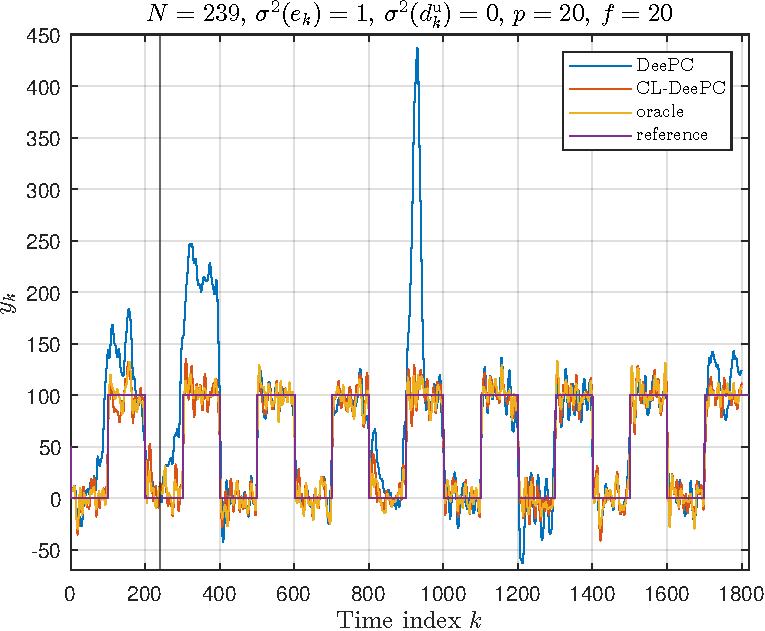
\includegraphics[width=\columnwidth]{results/figures/DeePC_CL_ID_issue_Re_1.mat_Nbar_239_p_20_f_20_Ru_1_Rdu_0_Q_100_R_0_dR_10.pdf}    % The printed column  
\caption{Reference tracking by adaptive \ac{DeePC} and \ac{CL-DeePC} using \ac{IVs}. After the vertical line at $\bar{N}$ all used data originates from operation in closed-loop. \ac{DeePC} displays worse reference tracking performance than \ac{CL-DeePC}, in part due to a closed-loop identification problem.}  % width is 8.4 cm.
\label{fig:CL_Problem_Solution}                                 % Size the figures 
\end{center}                                 % accordingly.
\end{figure}
% -----------------------------------------------------------

\subsection{Correlation between inputs and noise}
This section demonstrates the existence of correlation between inputs and preceding noise during closed-loop operation in an adaptive setting by means of simulations. Following the preceding consistency proof in \secref{sec:proof_IVs}, the correlation matrix of interest is given by $\frac{1}{N}E_{i_p,f_\mathrm{ID},N}\begin{bmatrix}U_{i,p,N}^\top & U_{i_p,f_\mathrm{ID},N}^\top\end{bmatrix}$, with $f_\mathrm{ID}=f$ for \ac{DeePC}, and $f_\mathrm{ID}=1$ for \ac{CL-DeePC}. An example of such a correlation matrix, averaged over 120 simulations with different noise realizations is shown by Fig.~\ref{}.
% ------------------------- Figure --------------------------
\begin{figure}[b!]
\begin{center}
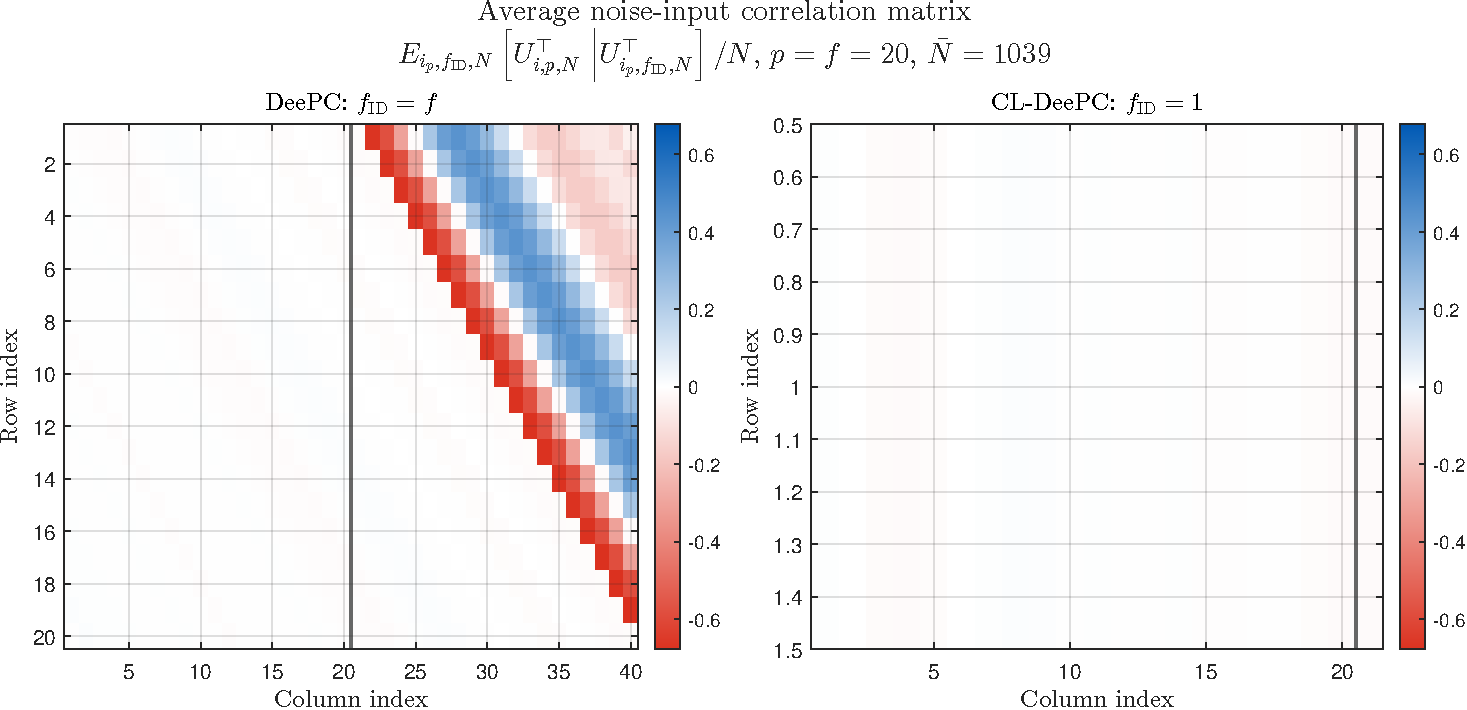
\includegraphics[width=\columnwidth]{results/figures/Correlation_Nbar_1039_p_20_f_20_Re_1_Ru_1_Rdu_0_Q_100_R_0_dR_10.pdf}    % The printed column  
\caption{Reference tracking by adaptive \ac{DeePC} and \ac{CL-DeePC} using \ac{IVs}. After the vertical line at $\bar{N}$ all used data originates from operation in closed-loop. \ac{DeePC} displays worse reference tracking performance than \ac{CL-DeePC}, in part due to a closed-loop identification problem.}  % width is 8.4 cm.
\label{fig:CL_Problem_Solution}                                 % Size the figures 
\end{center}                                 % accordingly.
\end{figure}
% -----------------------------------------------------------